\section{Diseño Estético del Prototipo}

\par 
El diseño estético del prototipo básicamente es el diseño del armazón o carcasa que cubrirá o encapsulara lo que es la placa y pantalla LCD del prototipo. Una vez diseñado el armazón se procederá a utilizar una impresora 3D para poder hacer nuestro diseño un objeto tangible. El proceso va a constar de realizar distintas iteraciones de un diseño del armazón e imprimirlo, una y otra vez hasta conseguir el armazón deseado. 

\subsection{Dimensiones del Prototipo}

\par 
Las medidas de nuestro prototipo son las siguientes:

\begin{figure}[H]
	\centering
	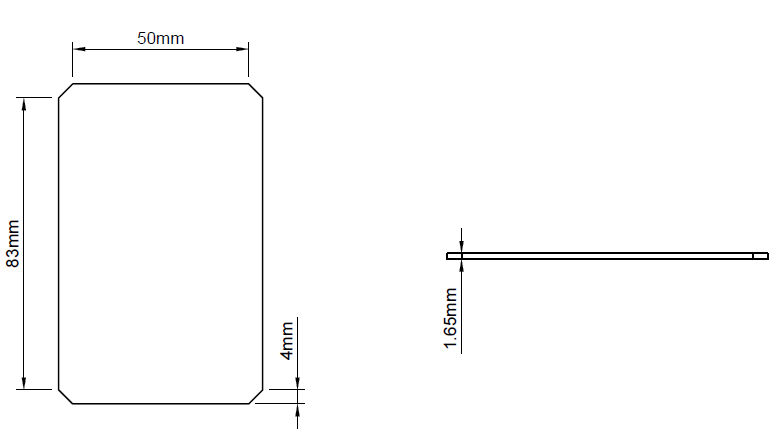
\includegraphics[width=0.8\linewidth]{mediciones1.png}
	\caption{Dibujo y dimensiones de la placa o circuito impreso}
\end{figure}

\par \noindent
Las dimensiones de nuestra placa es lo mas importante a la hora de hacer el armazón. En nuestra placa se encontrara el Arduino con sus respectivos módulos y componentes como resistencias, capacitores, interruptor, entrada jack de 3.5 mm y las conexiones con la pantalla LCD. Recordemos que la pantalla LCD viene en su propia placa; lo que requiere saber sus dimensiones.

\begin{figure}[H]
	\centering
	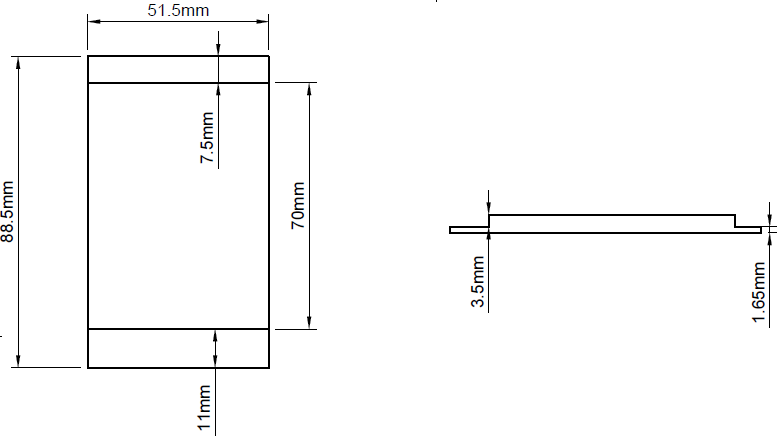
\includegraphics[width=0.8\linewidth]{mediciones2.png}
	\caption{Dibujo y dimensiones de la pantalla LCD y su respectiva placa}
\end{figure}

\par \noindent
Siendo la primera iteración de nuestro prototipo se decidió tener una placa para el circuito impreso y otra placa con el LCD. Esto es para que la pantalla LCD actué como una pieza modular del resto. La conexión de la pantalla LCD con el circuito sera a través de pines. Estos pines le dan una altura a nuestro LCD con respecto al circuito, como resultados todos los componentes del circuito se encuentran abajo de la placa LCD. El Armazón por lo tanto debe ser en base a lo siguiente:

\begin{figure}[H]
	\centering
	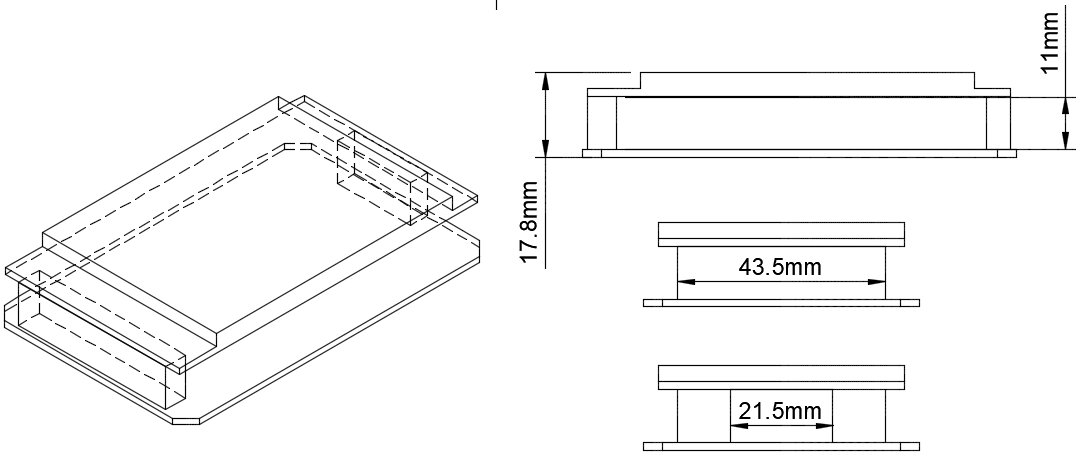
\includegraphics[width=0.8\linewidth]{mediciones3.png}
	\caption{Prototipo ensamblado, base para el diseño del armazón}
\end{figure}
